\documentclass[tikz,border=10pt]{standalone}
\begin{document}
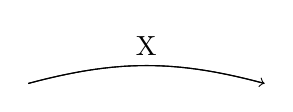
\begin{tikzpicture}
  \coordinate (a) at (0,0);
  \coordinate (b) at (3,0);
  \draw (a) to[bend left=15] node[inner sep=0pt, circle, name=M] {} (b);
  \draw[->] (a) to[bend left=15] node[above, name=L] {X} (b);
  \makeatletter
  \pgf@process{\pgfpointanchor{M}{center}}
  \typeout{P15-0 M,\the\pgf@x,\the\pgf@y}
  \pgf@process{\pgfpointanchor{L}{center}}
  \typeout{P15-0 L,\the\pgf@x,\the\pgf@y}
  \pgf@process{\pgfpointanchor{L}{south}}
  \typeout{P15-0 S,\the\pgf@x,\the\pgf@y}
  \makeatother
\end{tikzpicture}
\end{document}
